% preamble for the RiTeh thesis template

\documentclass[botnum,a4paper,11,oneside,final]{tex_aux/rithesis}
%\usepackage[latin1]{inputenc}
%\usepackage[T1]{fontenc}
%\usepackage[english]{babel}
%%%%%%% adjustment for croatian
\usepackage[croatian]{babel}
\usepackage[cp1250]{inputenc}	% this ensures croatian special letters are correctly printed with Windows

\usepackage{graphicx}	% this enables import of graphics
\usepackage[labelsep=space,format=hang]{caption}  % adjusts caption style
\usepackage{subfig}	% this enables use of subfigures
\usepackage{amsmath}
\usepackage{amssymb}
%\usepackage{fancyhdr}
\usepackage{amsfonts}
%\usepackage{amsthm}
%\usepackage{pdfsync}
% This package is used to tell TeXShop where things are in the PDF file.
% Command-click at any spot in the PDF and it will jump to the corresponding
% location in the source file.
\usepackage{epsfig}		% to use eps figures; maybe not necessary to use here with Mac
\usepackage{epstopdf}	% this automatically converts any eps-figure into a pdf-figure
\usepackage[section]{placeins} % da slika ne upada u sljedeci section

\hyphenation{sko-ko-vi-toj}

\DeclareGraphicsRule{.tif}{png}{.png}{`convert #1 `dirname #1`/`basename #1 .tif`.png}	% this converts any tif-figure into a png-figure (Mac directly supports pdf, jpg, png, and mps formats, but additionally can use tif and eps when they are automatically converted in png, and pdf, respectively, using the above two packages
\DeclareGraphicsExtensions{.pdf,.jpeg,.jpg,.png}  % ekstenzije koje ne treba pisati uz ime slike
\graphicspath{{slike/}}   % mjesto gdje su smjestene slike

%\usepackage{makeidx}	% this enables creation of index
%\usepackage{showidx}
%\makeindex			% this makes index automatically, based on author's entries

%\usepackage{eufrak}
%\usepackage[mathcal]{euscript}
\usepackage{psfrag}
%\usepackage{url} 
\usepackage{hyperref}
\hypersetup{
breaklinks,
colorlinks=true,
linkcolor=black,
citecolor=black,
filecolor=black,
urlcolor=black
}

\setcounter{topnumber}{1} \setcounter{bottomnumber}{1}

\newcommand{\navod}[1]{``#1''}

%
%
%

% pomocu \includeonly moze se kompajlirati samo odredjeno poglavlje, da se skrati vrijeme kompajliranja, dok se ne isprave pogreske u tom poglavlju npr.:

%\includeonly{Poglavlje_2}


\begin{document}

\frontmatter   % - ne dirati

% upisati naziv studija
\degreesubject{Diplomski studij ra�unarstva} % upisati odgovarajuci naziv studija

% upisati vrstu rada
\documenttype{Diplomski rad}  % Zavrsni rad ili Diplomski rad

\title{Ispitivanje Near Field Communication i Bluetooth Low Energy tehnologija na Android ure\dj ajima}   % upisati specificni naslov rada

\date{Svibanj, \thisyear.}   % upisati samo aktualni mjesec predaje rada

\author{Dino Biki\'{c}}  % upisati svoje ime i prezime
\jmbag{0069053128}  % upisati vlastiti JMBAG
\maketitle		% ne dirati

%\makecopyright

% Okruzenje za pisanje posvete. Maknuti komentare ukoliko se �eli napisati posvetu.
%\begin{dedication}
	%Ovo je posveta nekome
%\end{dedication}

% Okruzenje za pisanje zahvale
%\begin{acknowledgments} % maknuti komentare ukoliko se �eli napisati zahvalu
	%\include{Zahvala}  
	% tekst upisati u datoteku ``Zahvala'' i ukloniti komentar ili ga upisati izravno ovdje
%\end{acknowledgments}

\mentor{doc.dr.sc.~Miroslav Joler}   % zamijeniti podacima o svojem mentoru
\maketitleabstract

% kreira mjesto za umetnuti stranicu s opisom zadatka - ne dirati
\begin{assignmentpage}
\end{assignmentpage}

% kreira mjesto za umetnuti stranicu s izjavom o samostalnoj izradbi zadatka - ne dirati
\begin{honestystatementpage}
\end{honestystatementpage}

% kreiranje popisa sadrzaja, slika i tabela - ni�ta ne dirati
\tableofcontents
\listoffigures
\listoftables

% Lista kratica koristenih u tekstu. Kratice upisati u datoteku ``Kratice.tex'' koja je prilozena u paketu.
% Nije obavezno. Ako se ne zeli koristiti, onda ovaj blok staviti u komentar pomocu znaka %
\begin{glossary}{Longest string}
	% ovo je primjer koristenja, a student neka to zamijeni svojim kraticama i doda sve koje zeli
% ako se ne zeli deklarirati popis kratica, onda ga staviti pod komentar u glavnoj datoteci

   \item[{\bf 3DES}]	Triple Data Encryption Algorithm
   \item[{\bf AES}]	Advanced Encryption Standard
   \item[{\bf API}]	Application Program Interface
   \item[{\bf ART}]	Android Runtime
   \item[{\bf ASK}]	Amplitude-Shift Keying
   \item[{\bf BLE}]	Bluetooth Low Energy
   \item[{\bf BLP}]	Blood Pressure Profile 
   \item[{\bf CMS}]	Content Management System
   \item[{\bf CSCP}]	Cycling Speed and Cadence Profile
   \item[{\bf CSS}]	Cascading Style Sheets
   \item[{\bf ESN}]	Electronic Serial Number
   \item[{\bf FAB}]	Floating Action Button
   \item[{\bf FeliCa}]	Felicity Card
   \item[{\bf FMP}]	Find Me Profile
   \item[{\bf GAP}]	Generic Access Profile
   \item[{\bf GATT}]	Generic Attribute Profile 
   \item[{\bf GFSK}]	Gaussian Frequency Shift Modulation
   \item[{\bf GSM}]	Global System for Mobile Communications
   \item[{\bf GLP}]	Glucose Profile
   \item[{\bf HID }]	Human Interface Device
   \item[{\bf HOGP }]	HID over GATT Profile
   \item[{\bf HRP }]	Heart Rate Profile 
   \item[{\bf HTML }]	Hypertext Markup Language
   \item[{\bf HTTP }]	Hypertext Transfer Protocol
   \item[{\bf IMEI }]	International Mobile Station Equipment Identity
   \item[{\bf JSON }]	JavaScript Object Notation
   \item[{\bf MEID}]	Mobile Equipment Identifier
   \item[{\bf MVP}]	Model View Presenter
   \item[{\bf NDEF}]	NFC Data Exchange Format
   \item[{\bf NFC}]	Near Field Communication
   \item[{\bf PHP}]	Hypertetxt Preprocessor
   \item[{\bf POI}]	Point of Interes
   \item[{\bf PXP}]	Proximity Profile
   \item[{\bf RFID}]	Radio-Frequency Identification
   \item[{\bf SDK}]	Software Developtment Kit 
   \item[{\bf SFTP}]	Secure File Transfer Protocol
   \item[{\bf SIG}]	Bluetooth Special Interest Group
   \item[{\bf SQL}]	Structured Querry Language
   \item[{\bf URI}]	Uniform Resource Identifier
   \item[{\bf XML}]	Extensible Markup Language
   \item[{\bf VM}]	Virtual Machine
\end{glossary}

% kreiranje glavnoga dijela rada
\mainmatter		% ne dirati


% Ovdje pomo�u include funkcije ucitavati kreirana poglavlja. Poglavljima dajte logicna imena s obzirom na sadrzaj prikazan u njima (bez razmaka u imenu).
\chapter{Kako koristiti paket za pisanje Zavr�noga rada u \LaTeX-u}
Ovo su uvodne napomene za kori�tenje predlo�ka za pisanje Zavr�noga ili Diplomskoga rada studenata Tehni�koga fakulteta u Rijeci.

Paket je pripremljen tako da student �to prije mo�e pisati vlastiti tekst u ve� pripremljenom predlo�ku koji �e, uz minimalno u�enje sintakse \LaTeX-a, studentu olak�ati urediti svoj rad. U paketu su uklju�ene potrebne upute i sintakti�ke strukture koje bi trebale udovoljiti potrebama ve�ine studenta, a dodatne informacije postoje u priru�nicima odnosno na web stranicama na internetu koje su posve�ene \LaTeX-u (vidi u nastavku).

{\color{red} POZOR: paket treba biti prekopiran negdje na disk ne mijenjaju�i originalnu strukturi mapa (foldera) i ne mijenjaju�i nazive datoteka koje su u mapi \emph{tex\_aux}!}

\section{Opis sadr�aja paketa}
Paket se sastoji od
\begin{itemize}
 \item datoteke \href{UPUTE.pdf}{\emph{UPUTE.pdf}} koja sadr�i postupak instalacije potrebnih alata na ra�unalo te kori�tenja paketa. \emph{UPUTE} su bazirane na Windows OS, a korisnici drugih OS si na nazna�enim web lokacijama samo trebaju na�i instalacije za njihov OS.
 \item \verb|JMBAG_Ime_Prezime.tex| datoteke koja je sredi�nja datoteka koja povezuje sve cjeline i kompajliranjem koje se dobije izlazni \verb|JMBAG_Ime_Prezime.pdf| dokument.\\ U ovoj se datoteci inicijalno nalaze i upute za kori�tenje paketa kao i primjeri osnovne uporabe naj�e��ih sintakti�kih struktura u \LaTeX-u koje bi trebale biti dovoljne ve�ini studenata za pisanje rada.
 %
 \item \verb|tex_aux| mape u kojoj su interne datoteke koje definiraju stilove i dr. Student s njima ne treba \emph{ni�ta} raditi, ali one trebaju biti u \verb|tex_aux| mapi pod glavnom mapom Zavr�noga rada, kao �to je postavljeno u ovom paketu
 %
 \item mape \emph{slike} u koju student treba pohraniti sve slike koje �e koristiti u radu. Ime mape se ne smije preimenovati bez boljega poznavanja sintakse \LaTeX-a jer ovaj paket da bi ispravno radio o�ekuje ba� takvo ime mape
 %
 \item datoteke \verb|sintaksa_cestih_struktura.tex| koja ne sudjeluje izravno u kompajliranju pdf dokumenta, nego slu�i kao repozitorij u kojem su sadr�ane naj�e��e potrebne sintakti�ke strukture koje su spremne za kopiranje uz minimalnu prilagodbu parametara u studentovu radu
 %
 \item mape \href{run:manuals}{{\color{blue}manuals}} u kojoj se nalazi nekoliko najpopularnijih priru�nika za uporabu \LaTeX-a. 
\end{itemize}
%%%%%%%%%%%%%%%%%%%%%%%%%%%%%%%%%%%%%%%%%%%%%%%%%%%%%%%%%%%%%%%

\section{�ime se opremiti za pisanje rada}
Da bi se rad napisao pomo�u \LaTeX-a (a vrijedi svake lipe!), najprije je na ra�unalo potrebno instalirati (barem) \LaTeX~ software, a uz to, premda nije nu�an za pisanje rada, preporu�am i \emph{JabRef} software koji pomo�u intuitivnih su�elja korisniku omogu�ava kreiranje popisa literature na vrlo sofisticirani na�in. 

\subsection{Instalacija \LaTeX-a}
\begin{enumerate}
	\item odite na sredi�nji \LaTeX~ portal: \url{http://www.latex-project.org/}
	\item kliknite na poveznicu \href{http://www.latex-project.org/ftp.html}{Getting LaTeX} i potom uo�ite i povucite instalaciju koja odgovara va�em OSu (npr.\ proTeXt za Windows, MacTeX za Mac, TeX Live za Linux). Pozor: download je velik i mo�e du�e potrajati �ak i na brzoj vezi---dajte si dovoljno vremena za obaviti download.
	\item Instalirajte \LaTeX~ nabavljen u prethodnoj to�ki slijede�i upute koje su date za tu instalaciju (npr. proTeXt za Windowse daje kratki pdf s uputama koje vas vode kroz instalaciju korak po korak).
	\item Instalirajte si tekst-editor koji je pogodan za pisanje \LaTeX~ koda (npr.\ za Windows je popularan TeXnicCenter i dolazi ve� upakiran u proTeXt-u, za Mac je kvalitetan TeXShop koji sada tako�er dolazi u paketu s MacTeX-om).
\end{enumerate}

\subsection{Instalacija \emph{JabRef} softvera}
\emph{JabRef} je legalno besplatno dostupni softver za Windows OS (za druge OS �ete isto na�i takve programe) koji nam omogu�ava opisivanje literature na lak na�in pomo�u intuitivnih su�elja, a kao rezultat kreira \emph{BibTeX} datoteku \emph{ime.bib} (gdje je \emph{ime} koje korisnik proizvoljno dodijeli pri pohrani) u kojoj je literatura opisana na na�in koji \LaTeX~ razumije i na osnovi toga automatski formira popis literature na kraju na�ega rada, a sukladno redoslijedu pozivanja pojedine literature u tekstu.

\emph{Napomena: Kori�tenje BiBTeX programa kakav je \emph{JabRef} nije neophodno, ali prakti�no je. Alternativni---lo�iji---na�in jest ru�no opisati kori�tenu literaturu unutar \emph{tex} datoteke.\\ U datoteci po imenu \href{run:Literatura.tex}{{\color{blue}Literatura.tex}} koja je uklju�ena u ovaj paket ve� su namje�tene postavke kao da �e se literatura opisati pomo�u BiBTeX programa (npr.\ JabRef) i ne treba ni�ta mijenjati, a ispod toga se mo�e pro�itati upute i za drugi na�in (p)opisivanja literature.}

Instalacijska datoteka za \emph{JabRef} se mo�e prona�i na webu na adresi \url{http://jabref.sourceforge.net/}.
Preporu�eni postupak:
\begin{enumerate}
	\item povucite si i instalirajte posljednju stabilnu verziju \emph{JabRef}-a
	\item inicijalno se upoznajte s najva�nijim opcijama u \emph{JabRef}-u:
	\begin{enumerate}
		\item uo�ite ikonu (pod znakom ``+'' i tekstom \emph{New BibTeX Entry}) za unos nove jedinice literature (npr. knjige, �lanka, web portala i sl.)
		\item kada kliknete za unos nove stavke literature, uo�ite kakvi se sve tipovi literature nude za odabir. Odabirom opcije koja odgovara naslovu koji �elite unijeti, otvorit �e vam se novi prozor s poljima u koja se mo�e unijeti informacije o literaturi. Za odabrani tip literature samo su neka polja obavezna (nalaze se pod karticom (eng.\ \emph{tabom}) \emph{Required fields}), dok se pod drugim karticama mo�e i ne mora unijeti dodatne informacije.
		\item prije nego pohranite va� unos sa \emph{Ctrl+S}, morate toj jedinici dodijeliti jedinstveni identifikator, tzv.\ \emph{Bibtexkey}, �to je jedno od polja koja su obavezna za unos. Mo�ete ru�no upisati neki proizvoljni string, ali pogodnije je generirati ga automatski. Za to u�initi me�u ikonama na vrhu imate ikonu koja izgleda kao (�arobni) �tapi� sa zvjezdicama oko njega, klikom na kojega \emph{JabRef} automatski dodijeli jedinstveni BibTeX \emph{klju�} za tu bibliografsku jedinicu. Pomo�u toga klju�a se poslije bilo kada i bilo gdje u pisanju va�ega rada mo�ete pozvati na tu referencu, a \LaTeX~ �e sve ostalo obaviti za vas tj.\ dodijeliti joj odgovaraju�i broj u tekstu i s tim brojem uvrstiti u popis literature.
		\item korisnik ima mogu�nost i promijeniti uzorak po kojem se kreira struktura automatski generiranoga jedinstvenoga BibTeX klju�a tako da se ode u opciju izbornika \emph{Options $>>$ Preferences $>>$ BibTeX key generator} gdje je na vrhu prozora prikazan \emph{default} uzorak, npr. \verb|[auth]:[year]| �to zna�i da se klju� kreira na bazi \verb|prezime(autora):godina(rada)|. To se sada mo�e urediti po nekom novom uzorku, no ovako definirani uzorak u biti zadovoljava, a ako igdje ima potrebe za dodatnim razlikovanjem, mo�e se automatski generiran klju� jo� ru�no napraviti korekcija dodavanjem na kraju npr.\ \verb|_a| itd.
		\item klikom na karticu \emph{BibTeX source} mo�ete vidjeti kako �e unos va�ih podataka zapravo biti zapisan u va�oj \emph{ime.bib} datoteci koja �e se formirati od svih bibliografskih jedinica koje unesete.
		\item Za \emph{ime} va�e bibliografske datoteke kod pohrane odaberite \emph{Literatura} jer to ime o�ekuje ovaj paket. Ina�e se mo�e dodijeliti proizvoljno ime, ali onda treba znati �to i gdje promijeniti u sredi�njoj \LaTeX~ datoteci. Pozor: Datoteka \emph{Literatura.bib} koju ste tako kreirali mora se nalaziti unutar mape ovoga paketa da bi sve ispravno radilo! U paketu je za primjer ve� kreirana jedna datoteka istoga imena koju za vje�bu student mo�e i otvoriti u \emph{JabRef}-u, ali to su samo pokazne bibliografske jedinice unesene kao primjer, koje student treba u kona�nici zamijeniti svojim stvarnim podacima.
	\end{enumerate}
\end{enumerate} 
%%%%%%%%%%%%%%%%%%%%%%%%%%%%%%%%%%%%%%%%%%%%%%%%%%%

\section{Kako (kona�no) po�eti pisati svoj rad}
Najbr�i start je sljede�i:
\begin{enumerate}
	\item Pokrenite va� \LaTeX~tekst-editor i iz njega otvorite pripremljeni predlo�ak za pisanje rada \href{run:JMBAG_Ime_Prezime.tex}{{\color{blue}JMBAG\_Ime\_Prezime.tex}} koji se nalazi unutar ovoga paketa (obi�no ga se mo�e otvoriti i dvostrukim klikom na \emph{tex} datoteku ukoliko �e OS koristiti \LaTeX~ editor za otvaranje iste)
	\item skrolajte niz dokumentu ni�ta ne mijenjaju�i, dok ne nai�ete na retke u kojima su kratke upute koje upu�uju studenta �to treba upisati u pripremljenu naredbu. U biti, u gornjem dijelu dokumenta nema u biti ni�ega za mijenjati, nego tek nakon linije koja sadr�i \verb|\begin{document}|. Specifi�ni podaci koje student treba upisati bit �e uz naredbe:
	%
		\begin{itemize}
			\item \verb|\degreesubject|: upisati vrstu studija (preddiplomski ili diplomski studij studentovoga usmjerenja)
			\item \verb|\documenttype|: upisati \emph{Zavr�ni rad} ili \emph{Diplomski rad}
			\item \verb|\title|: upisati naslov rada
			\item \verb|\date|: upisati samo mjesec predaje rada. Godina se upisuje automatski.
			\item \verb|\author|: upisati ime i prezime studenta
			\item \verb|\jmbag|: zamijeniti postoje�i broj vlastitim JMBAG brojem 
			\item \verb|\mentor|: upisati titulu i ime i prezime svojega mentora
		\end{itemize}
	%
	\item Za prvu probu nakon une�enih podataka, kompajlirajte dokument na na�in da unutar va�ega tekst-editora odaberete opciju izbornika (odnosno ikonu) koja glasi ne�to poput \emph{Build and View (Current File)}. To pokrene postupak kompajliranja svega i rezultat bi trebao biti \emph{pdf} datoteka u kojoj �ete vidjeti lijepo formatirane po�etne stranice rada. Pozor: 
		\begin{itemize}
			\item provjerite u postavkama editora da je izlazni format PDF. To se ili vidi negdje na ekranu va�ega editora ili negdje pod opcijom koja glasi poput \emph{Select Output Profile} (vjerojatno pod \emph{Build} izbornikom) i nudi par izlaznih formata jedan od kojih je PDF.
			\item nekada je potrebno 2-3 puta pokrenuti \emph{Build} operaciju da bi sve promjene bile a�urirane u \emph{pdf} dokumentu kao �to su npr.\ brojevi referenca, popis literature i sl.
		\end{itemize}
		%
	\item Za (i vi�e nego) osnovnu sintaksu mo�ete otvoriti datoteku \href{run:Intro.tex}{{\color{blue}Intro.tex}} koja je dio paketa i unutar koje su napisane i ove upute. Vidjet �ete da da se odmah mo�e pisati va� tekst uz nekoliko osnovnih naredaba, kao �to su:
	\begin{itemize}
		\item \verb|\chapter{Naslov poglavlja}| kojim definirate naslov poglavlja
		\item \verb|\section{Naslov sekcije}| kojim definirate naslov sekcije unutar poglavlja
		\item \verb|\subsection{Naslov podsekcije}| kojim definirate naslov podsekcije
		\item \verb|\cite{bibtexkey}| kojom se pozivate na odre�enu literaturu jedinstveni klju� koje je u BibTeX datoteci \href{run:Literatura.bib}{{\color{blue}Literatura.bib}} dan sa \emph{bibtex key}
		\item \verb|\emph{tekst}| naredbu kojom se pomo�u italic slova nagla�ava neka rije� ili fraza
		\item \verb|\href| ili \verb|\url| naredba kojom se kreira poveznica na neku URL adresu ili dokument (ne pretjerujte s tim, odnosno uop�e ne morate to koristiti u radu, nego za vanjske reference koristiti samo \verb|\cite{}| naredbu, a za unutra�nje reference (na dijelove teksta) kombinaciju naredbi \verb|\label{ID}| i \verb|\ref{ID}| gdje se prvu postavi na dio teksta na koji �emo se poslije referencirati, a drugu na mjestu s kojega se referenciramo)
		\item ostale sintakse kao �to su ubacivanje slike, tabele ili jednad�ba mo�ete na�i u datoteci \href{run:sintaksa_cestih_struktura.tex}{{\color{blue}sintaksa\_cestih\_struktura.tex}} koja je dio paketa. Odabrane se strukture mo�e kopirati i zalijepiti u va� tekst, uz minimalne prilagodbe kao �to su naziv slike, veli�ina slike, opis i ID slike, a analogno i za tabele i jednad�be.
		\item Kona�no, za vi�e detalja o bilo �emu, potra�ite informacije u priru�nicima koji su prilo�eni u mapi \href{run:manuals}{{\color{blue}manuals}} ili na webu, gdje se, me�u obiljem drugih informacija, nalaze i korisne \href{http://en.wikibooks.org/wiki/LaTeX/}{wiki stranice} o \LaTeX-u pomo�u kojih se obi�no brzo prona�e upute i zadovoljavaju�e rje�enje kojom sintaksom se mo�e urediti �eljeni dio teksta.
  	\end{itemize}
\item Savjet: svako poglavlje napi�ite u novoj datoteci koju imenujte prikladnim imenom (bez razmaka u imenu) i potom ih samo pozivajte iz glavnoga dokumenta \emph{JMBAG\_Ime\_Prezime.tex} pomo�u \verb|\include{ime_datoteke}| naredbe.
\end{enumerate}

Nadam se da �e vam ovaj dokument pomo�i u pripremi teksta va�ega rada i omogu�iti tro�iti glavninu vremena na sadr�aj rada, a manje na formatiranje rada jer to bi za vas sada trebao obaviti \LaTeX! 
No, fair-playa radi, potrebno je napomenuti i sljede�e: \LaTeX~ je vrlo osjetljiv na pogre�ke u sintaksi naredbi (da, ba� kao svaki programski jezik) pa vas mo�e povremeno zagnjaviti javljanjem pogre�ke koju nikako ne uspijevate uo�iti gdje je. Iskustvo kojim se izbjegava ta nelagoda jest sljede�e:
\begin{itemize}
	\item budite koncentrirani dok pi�ete \LaTeX~naredbe
	\item kompajlirajte tekst prije nego se skupi puno teksta jer tako �ete imati manje teksta za prekontrolirati u slu�aju pogre�ke
	\item ako niste sigurni ho�e li vam raditi neka naredba nakon pisanja, radije odmah kompajlirajte tekst da vidite �to �ete dobiti i rije�ite dvojbu, nego �ekati da se skupi jo� dubioza, kada �e biti te�e detektirati koja naredba zapravo izaziva probleme (\LaTeX~ov prozor s porukama nije odve� precizan u lociranju i opisu pogre�aka)
\end{itemize}

%%%%%%%% POGLAVLJE ZAVRSENO %%%%%%%%%%%%%%%


\chapter{Primjeri naj�e��ih sintakti�kih struktura}
Ovo se poglavlje u ovome trenutku i ne mora �itati, ali za one koje se �ele bolje pripremiti prije samoga po�etka pisanja rada, sigurno �e pomo�i. 

U nastavku su opisane naj�e��e sintakti�ke strukture, a koje za budu�e potrebe imate pohranjene i u datoteci \href{run:sintaksa_cestih_struktura.tex}{{\color{blue}sintaksa\_cestih\_struktura.tex}} koja je sastavni dio glavne mape ovoga paketa.

\section{Ubacivanje slike}
Na Slici~\ref{fig:prva} je prikazana osnovna shema HPM sustava.
\begin{figure}[!htbp]
	\begin{center}
 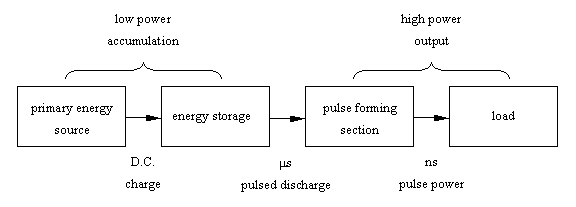
\includegraphics[height=4cm,width=8cm,keepaspectratio=true]{HPMsystem}
 \caption{Primjer ubacivanja slike}
 \label{fig:prva}
	\end{center}
\end{figure}

Znak \verb|~| iza rije�i Slici osigurava to�no jedan znak razmaka, �to poma�e ukoliko je rij�e Slika na kraju retka, da ne razdvoji rije� Slika i pripadaju�i broj slike.
Parametri slike \emph{width} i \emph{height} odre�uju maksimalne dopu�tene dimenzije pri �emu se primarno po�tuje manju navedenu dimenziju, a \emph{keepaspectratio} osigurava zadr�avanje odnosa dimenzija slike, odnosno sprje�ava deformaciju slike, nakon proizvoljno unesenih veli�ina.

Uo�i da sve oznake tj.\ \emph{labeli} ne smiju imati razmak u imenu. To vrijedi i op�enito, a ne samo za slike.

Tako�er, uo�i da nije potrebno pisati ekstenziju slike jer to je ure�eno u postavkama glavnoga dokumenta pa time �tedi trud. Ekstenzije koje se mo�e izostaviti su: \emph{jpg}, \emph{jpeg}, \emph{png} i \emph{pdf}.

Shema prikazana na Slici~\ref{fig:prva} �e biti kori�tena i za potrebe idu�ih primjera, a {\color{blue} u mapi na va�em disku ju obri�ite nakon �to po�nete pohranjivati vlastite slike vezane uz va� rad}.


\section{Ubacivanje podslika}
%
\begin{figure}[!htpb]
	  \begin{center}
	   \subfloat[kra�i opis podslike a]{\label{fig:HPM_a} 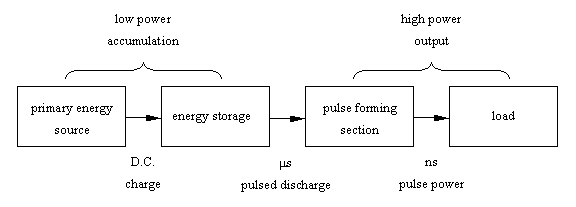
\includegraphics[height=5cm,width=8cm,keepaspectratio=true]{HPMsystem}} \\ %\hspace{10pt}
	   \subfloat[kra�i opis podslike b]{\label{fig:HPM_b} 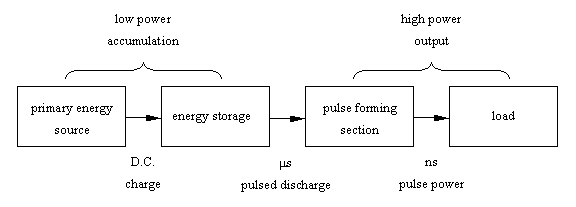
\includegraphics[height=5cm,width=8cm,keepaspectratio=true]{HPMsystem}}
\caption{Primjer ubacivanja vi�e podslika. Ovo je opis cijele slike.}
\label{fig:HPMsystem_2}
	  \end{center}
\end{figure}

Na Slici~\ref{fig:HPMsystem_2} su prikazane dvije podslike. 
Podslika~\ref{fig:HPM_a} pokazuje shemu HPM sustava, a podslika~\ref{fig:HPM_b} -- to isto.


\section{Ubacivanje tabele} \label{tabela}
Vi�e detalja o kreiranju tabela pro�itajte u literaturi, a sljede�i blok vam omogu�ava kreiranje jednostavne tabele, kao �to je prikazano u Tabeli~\ref{tab:prva}.
\begin{table}[!htbp]
\caption{Ovo je primjer izrade tabele}
\centering
\begin{tabular}{|c|c|c|}
\hline
variabla & vrijednost 1 & vrijednost 2  \\ [0.5ex]
\hline \hline  
A & 5 & 3 \\ [0.5ex]
B & 4 & 2 \\ [0.5ex]
\hline
\end{tabular}
\label{tab:prva}
\end{table}

Podaci koji su u stupcima se u tabeli razdvajaju znakom \&. Novi redak se na kraju aktualnoga retka formira znakom \verb|\\|. Broj stupaca se definira iza \emph{tabular} time �to se navedu slova koja ozna�avaju poravnavanje teksta u svakom stupcu, a broj slova zna�i broj stupaca koji �e biti kreiran u tabeli.


\section{Referenca na literaturu, sekciju, stranicu}
Na pojedinu se literaturu jednostavno uputi kori�tenjem naredbe \verb|\cite{bitex_key}| gdje je \emph{bibtex\_key} identifikator te bibliografske jedinice u bibtex datoteci. Npr.\ \verb|\cite{latex}| �e u tekstu pokazati broj te bibliografske jedinice u uglatoj zagradi \cite{latex}, te ju s istim brojem uvrsiti u popis literature (Bibliografiju) na kraju rada.

Ako se �elimo referirati na tekst u nekoj drugoj sekciji, kao npr. na dio gdje se opisuje kreiranje tabele, tada kraj te sekcije stavimo oznaku \verb|\label{ID}|, npr.\ \verb|\label{tabela}|, a na �eljenom mjestu u tekstu se na to referiramo pomo�u \verb|\ref{ID}|, npr.\ \verb|\ref{tabela}|. Tako mo�emo onda napisati da je kreiranje tabele opisano u Sekciji~\verb|~\ref{tabela}|, �to proizvede tekst koji glasi ``u Sekciji~\ref{tabela}''.

Ako �elimo navesti stranicu u na�em radu u kojoj se nalazi neki dio informacije o kojem govorimo, tada na isti na�in primijenimo \verb|\label{ID}| oznaku, a za referiranje na tu stranicu koristimo sintaksu \verb|\pageref{ID}|. 
Tako npr.\ mo�emo re�i da je primjer kreiranja tabele opisan na stranici~\verb|\pageref{tabela}|, �to �e za rezultat ima tekst u kojem pi�e da je primjer kreiranja tabele ``opisan na stranici~\pageref{tabela}''.

\section{Nagla�avanje teksta}
\subsection{Navodnici}
Za navodnike s lijeve strane fraze (otvaranje navodnika) koristi se 2x jednostruki navodnik koji se na tipkovnici nalazi lijevo od broja 1, a za navodnike s desne strane fraze (zatvaranja navodnika) se koristi 2x jednostruki navodnik koji se na tipkovnici nalazi na tipki \emph{�}, �to proizvede npr.\ ``abc''.

Alternativno, u ovom paketu je pripremljena i naredba \verb|\navod{abc}| gdje je \emph{abc} tekst koji se stavlja izme�u navodnika, tj.\ \navod{abc}.

\subsection{Kosa i podebljana slova}
Nagla�eni tekst (sli�no kosim slovima) mo�emo dobiti uporabom naredbe \verb|\emph{abc}| gdje je \emph{abc} neki tekst koji se �eli naglasiti.

Kosa slova (italic) mo�emo dobiti uporabom naredbe \verb|\textit{abc}| gdje je \textit{abc} neki tekst koji se �eli naglasiti.

Podebljana slova mo�emo posti�i uporabom naredbe \verb|\textbf{abc}| gdje je \textbf{abc} neki tekst koji �elimo podebljati.

\section{Verbatim okru�enje}
Verbatim okru�enje omogu�ava ispis teksta u izvornom obliku, bez da ga \LaTeX~ tuma�i po svojoj default sintaksi. To je pogodno kada se npr.\ na stranicu �eli kopirati dio programskoga koda iz nekog jezika i �elimo zadr�ati sve izvorne znakove, a ne da \LaTeX po�ne javljati pogre�ke kod kompajliranja jer �e ih bez toga interpretirati kao pogre�ke u sintaksi.

Postoji kra�i i du�i oblik verbatima. Kra�i slu�i za kra�u frazu od jedne ili par rije�i, a du�i za vi�e redaka.

Kra�i ima sintaksu: \verb+\verb|neka fraza|+

Du�i ima sintaksu:\\
\verb|\begin{verbatim}| \\
\verb|neki tekst| \\
\verb|\end{verbatim}| \\


\section{Kreiranje jedne jednad�be ili serije jednad�ba}

\subsection{Kreiranje jedne jednad�be}
Jednad�ba se napi�e u posebnom matemati�kom modu koji se kreira pomo�u bloka:
\begin{equation}
 A = B + C   \label{eq:prva}
\end{equation}

Jednad�ba~\eqref{eq:prva} je jedna jednostavna numerirana jednad�ba. Ako ju se ne �eli numerirati, onda se nakon rije�i \emph{begin} stavi zvjezdica, tj.\ \emph{begin\*}.

\subsection{Kreiranje vi�e jednad�ba}
Vi�e se jednad�ba kreira \emph{subequations} blokom:
\begin{subequations}
Dvije jednad�be mogu npr.\ glasiti:
\begin{align}
        A &= B + C  				\label{subeq:prva} \\
        D &= F + G				  \label{subeq:druga}
\end{align}
\label{subeq:obje}
\end{subequations}

U \eqref{subeq:prva} je prikazano dobivanje vrijednosti $A$, a u \eqref{subeq:druga} je prikazano dobivanje vrijednosti $D$. Jed.~\eqref{subeq:obje} je �uveni studentov zakon!

\section{Liste}
Liste su �este forme u tekstu kojima se na pregledni na�in nabrajaju neke stavke. Stavke obi�no navodimo s to�kama na po�etku, ili s brojevima ili sa slovima. U \LaTeX~u su upravo ta tri stila unaprijed definirana, a mogu�e su i slo�enije definicije stilova i kombinacije lista.

\subsection{Lista s to�kama}
Lista s to�kama se postigne blokom
\begin{verbatim}
\begin{itemize}
	\item prva stavka
	\item druga stavka
\end{itemize}
\end{verbatim}
�to na ekranu proizvede:
\begin{itemize}
	\item prva stavka
	\item druga stavka
\end{itemize}

\subsection{Numerirana lista s brojevima}
Numerirana lista s brojevima se postigne blokom
\begin{verbatim}
\begin{enumerate}
	\item prva stavka
	\item druga stavka
\end{enumerate}
\end{verbatim}
�to na ekranu proizvede:
\begin{enumerate}
	\item prva stavka
	\item druga stavka
\end{enumerate}


\subsection{Slov�ano numerirana lista}
Takva se lista mo�e posti�i u sklopu op�enitije forme koja omogu�uje proizvoljni opis ispred pojedine stavke, pomo�u sljede�ega bloka:
\begin{verbatim}
\begin{description}
	\item[a)] prva stavka
	\item[b)] druga stavka
\end{description}
\end{verbatim}
�to na ekranu proizvede:
\begin{description}
	\item[a)] prva stavka
	\item[b)] druga stavka
\end{description}



\section{Zavr�ne napomene}
Ovime zaklju�ujemo upute koje �e najve�em broju studenata biti dovoljne (ili barem dovoljna osnova) za uspje�no pisanje Zavr�noga odnosno Diplomskoga rada.

Prije nego prije�ete na kreiranje vlastitoga sadr�aja u�inite sljede�e:
\begin{enumerate}
	\item u mapi \href{run:slike}{{\color{blue}slike}}, obri�ite datoteku \verb|HPMsystem.png| jer je ona samo slu�ila za ilustracije u uputama
	%
	\item u glavnoj datoteci  \href{run:JMBAG\_Ime\_Prezime.tex}{{\color{blue}JMBAG\_Ime\_Prezime.tex}} stavite znak komentare ``\%'' ispred linije \verb|\chapter{Kako koristiti paket za pisanje Zavr�noga rada u \LaTeX-u}
Ovo su uvodne napomene za kori�tenje predlo�ka za pisanje Zavr�noga ili Diplomskoga rada studenata Tehni�koga fakulteta u Rijeci.

Paket je pripremljen tako da student �to prije mo�e pisati vlastiti tekst u ve� pripremljenom predlo�ku koji �e, uz minimalno u�enje sintakse \LaTeX-a, studentu olak�ati urediti svoj rad. U paketu su uklju�ene potrebne upute i sintakti�ke strukture koje bi trebale udovoljiti potrebama ve�ine studenta, a dodatne informacije postoje u priru�nicima odnosno na web stranicama na internetu koje su posve�ene \LaTeX-u (vidi u nastavku).

{\color{red} POZOR: paket treba biti prekopiran negdje na disk ne mijenjaju�i originalnu strukturi mapa (foldera) i ne mijenjaju�i nazive datoteka koje su u mapi \emph{tex\_aux}!}

\section{Opis sadr�aja paketa}
Paket se sastoji od
\begin{itemize}
 \item datoteke \href{UPUTE.pdf}{\emph{UPUTE.pdf}} koja sadr�i postupak instalacije potrebnih alata na ra�unalo te kori�tenja paketa. \emph{UPUTE} su bazirane na Windows OS, a korisnici drugih OS si na nazna�enim web lokacijama samo trebaju na�i instalacije za njihov OS.
 \item \verb|JMBAG_Ime_Prezime.tex| datoteke koja je sredi�nja datoteka koja povezuje sve cjeline i kompajliranjem koje se dobije izlazni \verb|JMBAG_Ime_Prezime.pdf| dokument.\\ U ovoj se datoteci inicijalno nalaze i upute za kori�tenje paketa kao i primjeri osnovne uporabe naj�e��ih sintakti�kih struktura u \LaTeX-u koje bi trebale biti dovoljne ve�ini studenata za pisanje rada.
 %
 \item \verb|tex_aux| mape u kojoj su interne datoteke koje definiraju stilove i dr. Student s njima ne treba \emph{ni�ta} raditi, ali one trebaju biti u \verb|tex_aux| mapi pod glavnom mapom Zavr�noga rada, kao �to je postavljeno u ovom paketu
 %
 \item mape \emph{slike} u koju student treba pohraniti sve slike koje �e koristiti u radu. Ime mape se ne smije preimenovati bez boljega poznavanja sintakse \LaTeX-a jer ovaj paket da bi ispravno radio o�ekuje ba� takvo ime mape
 %
 \item datoteke \verb|sintaksa_cestih_struktura.tex| koja ne sudjeluje izravno u kompajliranju pdf dokumenta, nego slu�i kao repozitorij u kojem su sadr�ane naj�e��e potrebne sintakti�ke strukture koje su spremne za kopiranje uz minimalnu prilagodbu parametara u studentovu radu
 %
 \item mape \href{run:manuals}{{\color{blue}manuals}} u kojoj se nalazi nekoliko najpopularnijih priru�nika za uporabu \LaTeX-a. 
\end{itemize}
%%%%%%%%%%%%%%%%%%%%%%%%%%%%%%%%%%%%%%%%%%%%%%%%%%%%%%%%%%%%%%%

\section{�ime se opremiti za pisanje rada}
Da bi se rad napisao pomo�u \LaTeX-a (a vrijedi svake lipe!), najprije je na ra�unalo potrebno instalirati (barem) \LaTeX~ software, a uz to, premda nije nu�an za pisanje rada, preporu�am i \emph{JabRef} software koji pomo�u intuitivnih su�elja korisniku omogu�ava kreiranje popisa literature na vrlo sofisticirani na�in. 

\subsection{Instalacija \LaTeX-a}
\begin{enumerate}
	\item odite na sredi�nji \LaTeX~ portal: \url{http://www.latex-project.org/}
	\item kliknite na poveznicu \href{http://www.latex-project.org/ftp.html}{Getting LaTeX} i potom uo�ite i povucite instalaciju koja odgovara va�em OSu (npr.\ proTeXt za Windows, MacTeX za Mac, TeX Live za Linux). Pozor: download je velik i mo�e du�e potrajati �ak i na brzoj vezi---dajte si dovoljno vremena za obaviti download.
	\item Instalirajte \LaTeX~ nabavljen u prethodnoj to�ki slijede�i upute koje su date za tu instalaciju (npr. proTeXt za Windowse daje kratki pdf s uputama koje vas vode kroz instalaciju korak po korak).
	\item Instalirajte si tekst-editor koji je pogodan za pisanje \LaTeX~ koda (npr.\ za Windows je popularan TeXnicCenter i dolazi ve� upakiran u proTeXt-u, za Mac je kvalitetan TeXShop koji sada tako�er dolazi u paketu s MacTeX-om).
\end{enumerate}

\subsection{Instalacija \emph{JabRef} softvera}
\emph{JabRef} je legalno besplatno dostupni softver za Windows OS (za druge OS �ete isto na�i takve programe) koji nam omogu�ava opisivanje literature na lak na�in pomo�u intuitivnih su�elja, a kao rezultat kreira \emph{BibTeX} datoteku \emph{ime.bib} (gdje je \emph{ime} koje korisnik proizvoljno dodijeli pri pohrani) u kojoj je literatura opisana na na�in koji \LaTeX~ razumije i na osnovi toga automatski formira popis literature na kraju na�ega rada, a sukladno redoslijedu pozivanja pojedine literature u tekstu.

\emph{Napomena: Kori�tenje BiBTeX programa kakav je \emph{JabRef} nije neophodno, ali prakti�no je. Alternativni---lo�iji---na�in jest ru�no opisati kori�tenu literaturu unutar \emph{tex} datoteke.\\ U datoteci po imenu \href{run:Literatura.tex}{{\color{blue}Literatura.tex}} koja je uklju�ena u ovaj paket ve� su namje�tene postavke kao da �e se literatura opisati pomo�u BiBTeX programa (npr.\ JabRef) i ne treba ni�ta mijenjati, a ispod toga se mo�e pro�itati upute i za drugi na�in (p)opisivanja literature.}

Instalacijska datoteka za \emph{JabRef} se mo�e prona�i na webu na adresi \url{http://jabref.sourceforge.net/}.
Preporu�eni postupak:
\begin{enumerate}
	\item povucite si i instalirajte posljednju stabilnu verziju \emph{JabRef}-a
	\item inicijalno se upoznajte s najva�nijim opcijama u \emph{JabRef}-u:
	\begin{enumerate}
		\item uo�ite ikonu (pod znakom ``+'' i tekstom \emph{New BibTeX Entry}) za unos nove jedinice literature (npr. knjige, �lanka, web portala i sl.)
		\item kada kliknete za unos nove stavke literature, uo�ite kakvi se sve tipovi literature nude za odabir. Odabirom opcije koja odgovara naslovu koji �elite unijeti, otvorit �e vam se novi prozor s poljima u koja se mo�e unijeti informacije o literaturi. Za odabrani tip literature samo su neka polja obavezna (nalaze se pod karticom (eng.\ \emph{tabom}) \emph{Required fields}), dok se pod drugim karticama mo�e i ne mora unijeti dodatne informacije.
		\item prije nego pohranite va� unos sa \emph{Ctrl+S}, morate toj jedinici dodijeliti jedinstveni identifikator, tzv.\ \emph{Bibtexkey}, �to je jedno od polja koja su obavezna za unos. Mo�ete ru�no upisati neki proizvoljni string, ali pogodnije je generirati ga automatski. Za to u�initi me�u ikonama na vrhu imate ikonu koja izgleda kao (�arobni) �tapi� sa zvjezdicama oko njega, klikom na kojega \emph{JabRef} automatski dodijeli jedinstveni BibTeX \emph{klju�} za tu bibliografsku jedinicu. Pomo�u toga klju�a se poslije bilo kada i bilo gdje u pisanju va�ega rada mo�ete pozvati na tu referencu, a \LaTeX~ �e sve ostalo obaviti za vas tj.\ dodijeliti joj odgovaraju�i broj u tekstu i s tim brojem uvrstiti u popis literature.
		\item korisnik ima mogu�nost i promijeniti uzorak po kojem se kreira struktura automatski generiranoga jedinstvenoga BibTeX klju�a tako da se ode u opciju izbornika \emph{Options $>>$ Preferences $>>$ BibTeX key generator} gdje je na vrhu prozora prikazan \emph{default} uzorak, npr. \verb|[auth]:[year]| �to zna�i da se klju� kreira na bazi \verb|prezime(autora):godina(rada)|. To se sada mo�e urediti po nekom novom uzorku, no ovako definirani uzorak u biti zadovoljava, a ako igdje ima potrebe za dodatnim razlikovanjem, mo�e se automatski generiran klju� jo� ru�no napraviti korekcija dodavanjem na kraju npr.\ \verb|_a| itd.
		\item klikom na karticu \emph{BibTeX source} mo�ete vidjeti kako �e unos va�ih podataka zapravo biti zapisan u va�oj \emph{ime.bib} datoteci koja �e se formirati od svih bibliografskih jedinica koje unesete.
		\item Za \emph{ime} va�e bibliografske datoteke kod pohrane odaberite \emph{Literatura} jer to ime o�ekuje ovaj paket. Ina�e se mo�e dodijeliti proizvoljno ime, ali onda treba znati �to i gdje promijeniti u sredi�njoj \LaTeX~ datoteci. Pozor: Datoteka \emph{Literatura.bib} koju ste tako kreirali mora se nalaziti unutar mape ovoga paketa da bi sve ispravno radilo! U paketu je za primjer ve� kreirana jedna datoteka istoga imena koju za vje�bu student mo�e i otvoriti u \emph{JabRef}-u, ali to su samo pokazne bibliografske jedinice unesene kao primjer, koje student treba u kona�nici zamijeniti svojim stvarnim podacima.
	\end{enumerate}
\end{enumerate} 
%%%%%%%%%%%%%%%%%%%%%%%%%%%%%%%%%%%%%%%%%%%%%%%%%%%

\section{Kako (kona�no) po�eti pisati svoj rad}
Najbr�i start je sljede�i:
\begin{enumerate}
	\item Pokrenite va� \LaTeX~tekst-editor i iz njega otvorite pripremljeni predlo�ak za pisanje rada \href{run:JMBAG_Ime_Prezime.tex}{{\color{blue}JMBAG\_Ime\_Prezime.tex}} koji se nalazi unutar ovoga paketa (obi�no ga se mo�e otvoriti i dvostrukim klikom na \emph{tex} datoteku ukoliko �e OS koristiti \LaTeX~ editor za otvaranje iste)
	\item skrolajte niz dokumentu ni�ta ne mijenjaju�i, dok ne nai�ete na retke u kojima su kratke upute koje upu�uju studenta �to treba upisati u pripremljenu naredbu. U biti, u gornjem dijelu dokumenta nema u biti ni�ega za mijenjati, nego tek nakon linije koja sadr�i \verb|\begin{document}|. Specifi�ni podaci koje student treba upisati bit �e uz naredbe:
	%
		\begin{itemize}
			\item \verb|\degreesubject|: upisati vrstu studija (preddiplomski ili diplomski studij studentovoga usmjerenja)
			\item \verb|\documenttype|: upisati \emph{Zavr�ni rad} ili \emph{Diplomski rad}
			\item \verb|\title|: upisati naslov rada
			\item \verb|\date|: upisati samo mjesec predaje rada. Godina se upisuje automatski.
			\item \verb|\author|: upisati ime i prezime studenta
			\item \verb|\jmbag|: zamijeniti postoje�i broj vlastitim JMBAG brojem 
			\item \verb|\mentor|: upisati titulu i ime i prezime svojega mentora
		\end{itemize}
	%
	\item Za prvu probu nakon une�enih podataka, kompajlirajte dokument na na�in da unutar va�ega tekst-editora odaberete opciju izbornika (odnosno ikonu) koja glasi ne�to poput \emph{Build and View (Current File)}. To pokrene postupak kompajliranja svega i rezultat bi trebao biti \emph{pdf} datoteka u kojoj �ete vidjeti lijepo formatirane po�etne stranice rada. Pozor: 
		\begin{itemize}
			\item provjerite u postavkama editora da je izlazni format PDF. To se ili vidi negdje na ekranu va�ega editora ili negdje pod opcijom koja glasi poput \emph{Select Output Profile} (vjerojatno pod \emph{Build} izbornikom) i nudi par izlaznih formata jedan od kojih je PDF.
			\item nekada je potrebno 2-3 puta pokrenuti \emph{Build} operaciju da bi sve promjene bile a�urirane u \emph{pdf} dokumentu kao �to su npr.\ brojevi referenca, popis literature i sl.
		\end{itemize}
		%
	\item Za (i vi�e nego) osnovnu sintaksu mo�ete otvoriti datoteku \href{run:Intro.tex}{{\color{blue}Intro.tex}} koja je dio paketa i unutar koje su napisane i ove upute. Vidjet �ete da da se odmah mo�e pisati va� tekst uz nekoliko osnovnih naredaba, kao �to su:
	\begin{itemize}
		\item \verb|\chapter{Naslov poglavlja}| kojim definirate naslov poglavlja
		\item \verb|\section{Naslov sekcije}| kojim definirate naslov sekcije unutar poglavlja
		\item \verb|\subsection{Naslov podsekcije}| kojim definirate naslov podsekcije
		\item \verb|\cite{bibtexkey}| kojom se pozivate na odre�enu literaturu jedinstveni klju� koje je u BibTeX datoteci \href{run:Literatura.bib}{{\color{blue}Literatura.bib}} dan sa \emph{bibtex key}
		\item \verb|\emph{tekst}| naredbu kojom se pomo�u italic slova nagla�ava neka rije� ili fraza
		\item \verb|\href| ili \verb|\url| naredba kojom se kreira poveznica na neku URL adresu ili dokument (ne pretjerujte s tim, odnosno uop�e ne morate to koristiti u radu, nego za vanjske reference koristiti samo \verb|\cite{}| naredbu, a za unutra�nje reference (na dijelove teksta) kombinaciju naredbi \verb|\label{ID}| i \verb|\ref{ID}| gdje se prvu postavi na dio teksta na koji �emo se poslije referencirati, a drugu na mjestu s kojega se referenciramo)
		\item ostale sintakse kao �to su ubacivanje slike, tabele ili jednad�ba mo�ete na�i u datoteci \href{run:sintaksa_cestih_struktura.tex}{{\color{blue}sintaksa\_cestih\_struktura.tex}} koja je dio paketa. Odabrane se strukture mo�e kopirati i zalijepiti u va� tekst, uz minimalne prilagodbe kao �to su naziv slike, veli�ina slike, opis i ID slike, a analogno i za tabele i jednad�be.
		\item Kona�no, za vi�e detalja o bilo �emu, potra�ite informacije u priru�nicima koji su prilo�eni u mapi \href{run:manuals}{{\color{blue}manuals}} ili na webu, gdje se, me�u obiljem drugih informacija, nalaze i korisne \href{http://en.wikibooks.org/wiki/LaTeX/}{wiki stranice} o \LaTeX-u pomo�u kojih se obi�no brzo prona�e upute i zadovoljavaju�e rje�enje kojom sintaksom se mo�e urediti �eljeni dio teksta.
  	\end{itemize}
\item Savjet: svako poglavlje napi�ite u novoj datoteci koju imenujte prikladnim imenom (bez razmaka u imenu) i potom ih samo pozivajte iz glavnoga dokumenta \emph{JMBAG\_Ime\_Prezime.tex} pomo�u \verb|\include{ime_datoteke}| naredbe.
\end{enumerate}

Nadam se da �e vam ovaj dokument pomo�i u pripremi teksta va�ega rada i omogu�iti tro�iti glavninu vremena na sadr�aj rada, a manje na formatiranje rada jer to bi za vas sada trebao obaviti \LaTeX! 
No, fair-playa radi, potrebno je napomenuti i sljede�e: \LaTeX~ je vrlo osjetljiv na pogre�ke u sintaksi naredbi (da, ba� kao svaki programski jezik) pa vas mo�e povremeno zagnjaviti javljanjem pogre�ke koju nikako ne uspijevate uo�iti gdje je. Iskustvo kojim se izbjegava ta nelagoda jest sljede�e:
\begin{itemize}
	\item budite koncentrirani dok pi�ete \LaTeX~naredbe
	\item kompajlirajte tekst prije nego se skupi puno teksta jer tako �ete imati manje teksta za prekontrolirati u slu�aju pogre�ke
	\item ako niste sigurni ho�e li vam raditi neka naredba nakon pisanja, radije odmah kompajlirajte tekst da vidite �to �ete dobiti i rije�ite dvojbu, nego �ekati da se skupi jo� dubioza, kada �e biti te�e detektirati koja naredba zapravo izaziva probleme (\LaTeX~ov prozor s porukama nije odve� precizan u lociranju i opisu pogre�aka)
\end{itemize}

%%%%%%%% POGLAVLJE ZAVRSENO %%%%%%%%%%%%%%%


\chapter{Primjeri naj�e��ih sintakti�kih struktura}
Ovo se poglavlje u ovome trenutku i ne mora �itati, ali za one koje se �ele bolje pripremiti prije samoga po�etka pisanja rada, sigurno �e pomo�i. 

U nastavku su opisane naj�e��e sintakti�ke strukture, a koje za budu�e potrebe imate pohranjene i u datoteci \href{run:sintaksa_cestih_struktura.tex}{{\color{blue}sintaksa\_cestih\_struktura.tex}} koja je sastavni dio glavne mape ovoga paketa.

\section{Ubacivanje slike}
Na Slici~\ref{fig:prva} je prikazana osnovna shema HPM sustava.
\begin{figure}[!htbp]
	\begin{center}
 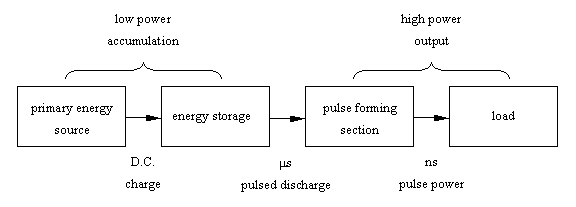
\includegraphics[height=4cm,width=8cm,keepaspectratio=true]{HPMsystem}
 \caption{Primjer ubacivanja slike}
 \label{fig:prva}
	\end{center}
\end{figure}

Znak \verb|~| iza rije�i Slici osigurava to�no jedan znak razmaka, �to poma�e ukoliko je rij�e Slika na kraju retka, da ne razdvoji rije� Slika i pripadaju�i broj slike.
Parametri slike \emph{width} i \emph{height} odre�uju maksimalne dopu�tene dimenzije pri �emu se primarno po�tuje manju navedenu dimenziju, a \emph{keepaspectratio} osigurava zadr�avanje odnosa dimenzija slike, odnosno sprje�ava deformaciju slike, nakon proizvoljno unesenih veli�ina.

Uo�i da sve oznake tj.\ \emph{labeli} ne smiju imati razmak u imenu. To vrijedi i op�enito, a ne samo za slike.

Tako�er, uo�i da nije potrebno pisati ekstenziju slike jer to je ure�eno u postavkama glavnoga dokumenta pa time �tedi trud. Ekstenzije koje se mo�e izostaviti su: \emph{jpg}, \emph{jpeg}, \emph{png} i \emph{pdf}.

Shema prikazana na Slici~\ref{fig:prva} �e biti kori�tena i za potrebe idu�ih primjera, a {\color{blue} u mapi na va�em disku ju obri�ite nakon �to po�nete pohranjivati vlastite slike vezane uz va� rad}.


\section{Ubacivanje podslika}
%
\begin{figure}[!htpb]
	  \begin{center}
	   \subfloat[kra�i opis podslike a]{\label{fig:HPM_a} 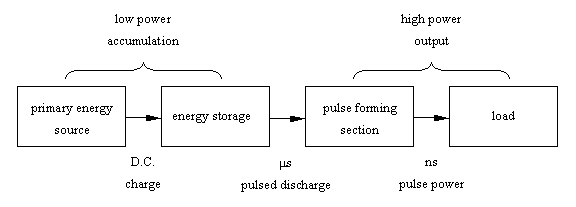
\includegraphics[height=5cm,width=8cm,keepaspectratio=true]{HPMsystem}} \\ %\hspace{10pt}
	   \subfloat[kra�i opis podslike b]{\label{fig:HPM_b} 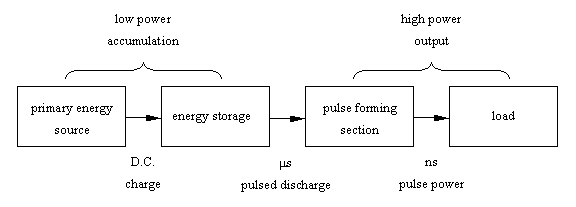
\includegraphics[height=5cm,width=8cm,keepaspectratio=true]{HPMsystem}}
\caption{Primjer ubacivanja vi�e podslika. Ovo je opis cijele slike.}
\label{fig:HPMsystem_2}
	  \end{center}
\end{figure}

Na Slici~\ref{fig:HPMsystem_2} su prikazane dvije podslike. 
Podslika~\ref{fig:HPM_a} pokazuje shemu HPM sustava, a podslika~\ref{fig:HPM_b} -- to isto.


\section{Ubacivanje tabele} \label{tabela}
Vi�e detalja o kreiranju tabela pro�itajte u literaturi, a sljede�i blok vam omogu�ava kreiranje jednostavne tabele, kao �to je prikazano u Tabeli~\ref{tab:prva}.
\begin{table}[!htbp]
\caption{Ovo je primjer izrade tabele}
\centering
\begin{tabular}{|c|c|c|}
\hline
variabla & vrijednost 1 & vrijednost 2  \\ [0.5ex]
\hline \hline  
A & 5 & 3 \\ [0.5ex]
B & 4 & 2 \\ [0.5ex]
\hline
\end{tabular}
\label{tab:prva}
\end{table}

Podaci koji su u stupcima se u tabeli razdvajaju znakom \&. Novi redak se na kraju aktualnoga retka formira znakom \verb|\\|. Broj stupaca se definira iza \emph{tabular} time �to se navedu slova koja ozna�avaju poravnavanje teksta u svakom stupcu, a broj slova zna�i broj stupaca koji �e biti kreiran u tabeli.


\section{Referenca na literaturu, sekciju, stranicu}
Na pojedinu se literaturu jednostavno uputi kori�tenjem naredbe \verb|\cite{bitex_key}| gdje je \emph{bibtex\_key} identifikator te bibliografske jedinice u bibtex datoteci. Npr.\ \verb|\cite{latex}| �e u tekstu pokazati broj te bibliografske jedinice u uglatoj zagradi \cite{latex}, te ju s istim brojem uvrsiti u popis literature (Bibliografiju) na kraju rada.

Ako se �elimo referirati na tekst u nekoj drugoj sekciji, kao npr. na dio gdje se opisuje kreiranje tabele, tada kraj te sekcije stavimo oznaku \verb|\label{ID}|, npr.\ \verb|\label{tabela}|, a na �eljenom mjestu u tekstu se na to referiramo pomo�u \verb|\ref{ID}|, npr.\ \verb|\ref{tabela}|. Tako mo�emo onda napisati da je kreiranje tabele opisano u Sekciji~\verb|~\ref{tabela}|, �to proizvede tekst koji glasi ``u Sekciji~\ref{tabela}''.

Ako �elimo navesti stranicu u na�em radu u kojoj se nalazi neki dio informacije o kojem govorimo, tada na isti na�in primijenimo \verb|\label{ID}| oznaku, a za referiranje na tu stranicu koristimo sintaksu \verb|\pageref{ID}|. 
Tako npr.\ mo�emo re�i da je primjer kreiranja tabele opisan na stranici~\verb|\pageref{tabela}|, �to �e za rezultat ima tekst u kojem pi�e da je primjer kreiranja tabele ``opisan na stranici~\pageref{tabela}''.

\section{Nagla�avanje teksta}
\subsection{Navodnici}
Za navodnike s lijeve strane fraze (otvaranje navodnika) koristi se 2x jednostruki navodnik koji se na tipkovnici nalazi lijevo od broja 1, a za navodnike s desne strane fraze (zatvaranja navodnika) se koristi 2x jednostruki navodnik koji se na tipkovnici nalazi na tipki \emph{�}, �to proizvede npr.\ ``abc''.

Alternativno, u ovom paketu je pripremljena i naredba \verb|\navod{abc}| gdje je \emph{abc} tekst koji se stavlja izme�u navodnika, tj.\ \navod{abc}.

\subsection{Kosa i podebljana slova}
Nagla�eni tekst (sli�no kosim slovima) mo�emo dobiti uporabom naredbe \verb|\emph{abc}| gdje je \emph{abc} neki tekst koji se �eli naglasiti.

Kosa slova (italic) mo�emo dobiti uporabom naredbe \verb|\textit{abc}| gdje je \textit{abc} neki tekst koji se �eli naglasiti.

Podebljana slova mo�emo posti�i uporabom naredbe \verb|\textbf{abc}| gdje je \textbf{abc} neki tekst koji �elimo podebljati.

\section{Verbatim okru�enje}
Verbatim okru�enje omogu�ava ispis teksta u izvornom obliku, bez da ga \LaTeX~ tuma�i po svojoj default sintaksi. To je pogodno kada se npr.\ na stranicu �eli kopirati dio programskoga koda iz nekog jezika i �elimo zadr�ati sve izvorne znakove, a ne da \LaTeX po�ne javljati pogre�ke kod kompajliranja jer �e ih bez toga interpretirati kao pogre�ke u sintaksi.

Postoji kra�i i du�i oblik verbatima. Kra�i slu�i za kra�u frazu od jedne ili par rije�i, a du�i za vi�e redaka.

Kra�i ima sintaksu: \verb+\verb|neka fraza|+

Du�i ima sintaksu:\\
\verb|\begin{verbatim}| \\
\verb|neki tekst| \\
\verb|\end{verbatim}| \\


\section{Kreiranje jedne jednad�be ili serije jednad�ba}

\subsection{Kreiranje jedne jednad�be}
Jednad�ba se napi�e u posebnom matemati�kom modu koji se kreira pomo�u bloka:
\begin{equation}
 A = B + C   \label{eq:prva}
\end{equation}

Jednad�ba~\eqref{eq:prva} je jedna jednostavna numerirana jednad�ba. Ako ju se ne �eli numerirati, onda se nakon rije�i \emph{begin} stavi zvjezdica, tj.\ \emph{begin\*}.

\subsection{Kreiranje vi�e jednad�ba}
Vi�e se jednad�ba kreira \emph{subequations} blokom:
\begin{subequations}
Dvije jednad�be mogu npr.\ glasiti:
\begin{align}
        A &= B + C  				\label{subeq:prva} \\
        D &= F + G				  \label{subeq:druga}
\end{align}
\label{subeq:obje}
\end{subequations}

U \eqref{subeq:prva} je prikazano dobivanje vrijednosti $A$, a u \eqref{subeq:druga} je prikazano dobivanje vrijednosti $D$. Jed.~\eqref{subeq:obje} je �uveni studentov zakon!

\section{Liste}
Liste su �este forme u tekstu kojima se na pregledni na�in nabrajaju neke stavke. Stavke obi�no navodimo s to�kama na po�etku, ili s brojevima ili sa slovima. U \LaTeX~u su upravo ta tri stila unaprijed definirana, a mogu�e su i slo�enije definicije stilova i kombinacije lista.

\subsection{Lista s to�kama}
Lista s to�kama se postigne blokom
\begin{verbatim}
\begin{itemize}
	\item prva stavka
	\item druga stavka
\end{itemize}
\end{verbatim}
�to na ekranu proizvede:
\begin{itemize}
	\item prva stavka
	\item druga stavka
\end{itemize}

\subsection{Numerirana lista s brojevima}
Numerirana lista s brojevima se postigne blokom
\begin{verbatim}
\begin{enumerate}
	\item prva stavka
	\item druga stavka
\end{enumerate}
\end{verbatim}
�to na ekranu proizvede:
\begin{enumerate}
	\item prva stavka
	\item druga stavka
\end{enumerate}


\subsection{Slov�ano numerirana lista}
Takva se lista mo�e posti�i u sklopu op�enitije forme koja omogu�uje proizvoljni opis ispred pojedine stavke, pomo�u sljede�ega bloka:
\begin{verbatim}
\begin{description}
	\item[a)] prva stavka
	\item[b)] druga stavka
\end{description}
\end{verbatim}
�to na ekranu proizvede:
\begin{description}
	\item[a)] prva stavka
	\item[b)] druga stavka
\end{description}



\section{Zavr�ne napomene}
Ovime zaklju�ujemo upute koje �e najve�em broju studenata biti dovoljne (ili barem dovoljna osnova) za uspje�no pisanje Zavr�noga odnosno Diplomskoga rada.

Prije nego prije�ete na kreiranje vlastitoga sadr�aja u�inite sljede�e:
\begin{enumerate}
	\item u mapi \href{run:slike}{{\color{blue}slike}}, obri�ite datoteku \verb|HPMsystem.png| jer je ona samo slu�ila za ilustracije u uputama
	%
	\item u glavnoj datoteci  \href{run:JMBAG\_Ime\_Prezime.tex}{{\color{blue}JMBAG\_Ime\_Prezime.tex}} stavite znak komentare ``\%'' ispred linije \verb|\chapter{Kako koristiti paket za pisanje Zavr�noga rada u \LaTeX-u}
Ovo su uvodne napomene za kori�tenje predlo�ka za pisanje Zavr�noga ili Diplomskoga rada studenata Tehni�koga fakulteta u Rijeci.

Paket je pripremljen tako da student �to prije mo�e pisati vlastiti tekst u ve� pripremljenom predlo�ku koji �e, uz minimalno u�enje sintakse \LaTeX-a, studentu olak�ati urediti svoj rad. U paketu su uklju�ene potrebne upute i sintakti�ke strukture koje bi trebale udovoljiti potrebama ve�ine studenta, a dodatne informacije postoje u priru�nicima odnosno na web stranicama na internetu koje su posve�ene \LaTeX-u (vidi u nastavku).

{\color{red} POZOR: paket treba biti prekopiran negdje na disk ne mijenjaju�i originalnu strukturi mapa (foldera) i ne mijenjaju�i nazive datoteka koje su u mapi \emph{tex\_aux}!}

\section{Opis sadr�aja paketa}
Paket se sastoji od
\begin{itemize}
 \item datoteke \href{UPUTE.pdf}{\emph{UPUTE.pdf}} koja sadr�i postupak instalacije potrebnih alata na ra�unalo te kori�tenja paketa. \emph{UPUTE} su bazirane na Windows OS, a korisnici drugih OS si na nazna�enim web lokacijama samo trebaju na�i instalacije za njihov OS.
 \item \verb|JMBAG_Ime_Prezime.tex| datoteke koja je sredi�nja datoteka koja povezuje sve cjeline i kompajliranjem koje se dobije izlazni \verb|JMBAG_Ime_Prezime.pdf| dokument.\\ U ovoj se datoteci inicijalno nalaze i upute za kori�tenje paketa kao i primjeri osnovne uporabe naj�e��ih sintakti�kih struktura u \LaTeX-u koje bi trebale biti dovoljne ve�ini studenata za pisanje rada.
 %
 \item \verb|tex_aux| mape u kojoj su interne datoteke koje definiraju stilove i dr. Student s njima ne treba \emph{ni�ta} raditi, ali one trebaju biti u \verb|tex_aux| mapi pod glavnom mapom Zavr�noga rada, kao �to je postavljeno u ovom paketu
 %
 \item mape \emph{slike} u koju student treba pohraniti sve slike koje �e koristiti u radu. Ime mape se ne smije preimenovati bez boljega poznavanja sintakse \LaTeX-a jer ovaj paket da bi ispravno radio o�ekuje ba� takvo ime mape
 %
 \item datoteke \verb|sintaksa_cestih_struktura.tex| koja ne sudjeluje izravno u kompajliranju pdf dokumenta, nego slu�i kao repozitorij u kojem su sadr�ane naj�e��e potrebne sintakti�ke strukture koje su spremne za kopiranje uz minimalnu prilagodbu parametara u studentovu radu
 %
 \item mape \href{run:manuals}{{\color{blue}manuals}} u kojoj se nalazi nekoliko najpopularnijih priru�nika za uporabu \LaTeX-a. 
\end{itemize}
%%%%%%%%%%%%%%%%%%%%%%%%%%%%%%%%%%%%%%%%%%%%%%%%%%%%%%%%%%%%%%%

\section{�ime se opremiti za pisanje rada}
Da bi se rad napisao pomo�u \LaTeX-a (a vrijedi svake lipe!), najprije je na ra�unalo potrebno instalirati (barem) \LaTeX~ software, a uz to, premda nije nu�an za pisanje rada, preporu�am i \emph{JabRef} software koji pomo�u intuitivnih su�elja korisniku omogu�ava kreiranje popisa literature na vrlo sofisticirani na�in. 

\subsection{Instalacija \LaTeX-a}
\begin{enumerate}
	\item odite na sredi�nji \LaTeX~ portal: \url{http://www.latex-project.org/}
	\item kliknite na poveznicu \href{http://www.latex-project.org/ftp.html}{Getting LaTeX} i potom uo�ite i povucite instalaciju koja odgovara va�em OSu (npr.\ proTeXt za Windows, MacTeX za Mac, TeX Live za Linux). Pozor: download je velik i mo�e du�e potrajati �ak i na brzoj vezi---dajte si dovoljno vremena za obaviti download.
	\item Instalirajte \LaTeX~ nabavljen u prethodnoj to�ki slijede�i upute koje su date za tu instalaciju (npr. proTeXt za Windowse daje kratki pdf s uputama koje vas vode kroz instalaciju korak po korak).
	\item Instalirajte si tekst-editor koji je pogodan za pisanje \LaTeX~ koda (npr.\ za Windows je popularan TeXnicCenter i dolazi ve� upakiran u proTeXt-u, za Mac je kvalitetan TeXShop koji sada tako�er dolazi u paketu s MacTeX-om).
\end{enumerate}

\subsection{Instalacija \emph{JabRef} softvera}
\emph{JabRef} je legalno besplatno dostupni softver za Windows OS (za druge OS �ete isto na�i takve programe) koji nam omogu�ava opisivanje literature na lak na�in pomo�u intuitivnih su�elja, a kao rezultat kreira \emph{BibTeX} datoteku \emph{ime.bib} (gdje je \emph{ime} koje korisnik proizvoljno dodijeli pri pohrani) u kojoj je literatura opisana na na�in koji \LaTeX~ razumije i na osnovi toga automatski formira popis literature na kraju na�ega rada, a sukladno redoslijedu pozivanja pojedine literature u tekstu.

\emph{Napomena: Kori�tenje BiBTeX programa kakav je \emph{JabRef} nije neophodno, ali prakti�no je. Alternativni---lo�iji---na�in jest ru�no opisati kori�tenu literaturu unutar \emph{tex} datoteke.\\ U datoteci po imenu \href{run:Literatura.tex}{{\color{blue}Literatura.tex}} koja je uklju�ena u ovaj paket ve� su namje�tene postavke kao da �e se literatura opisati pomo�u BiBTeX programa (npr.\ JabRef) i ne treba ni�ta mijenjati, a ispod toga se mo�e pro�itati upute i za drugi na�in (p)opisivanja literature.}

Instalacijska datoteka za \emph{JabRef} se mo�e prona�i na webu na adresi \url{http://jabref.sourceforge.net/}.
Preporu�eni postupak:
\begin{enumerate}
	\item povucite si i instalirajte posljednju stabilnu verziju \emph{JabRef}-a
	\item inicijalno se upoznajte s najva�nijim opcijama u \emph{JabRef}-u:
	\begin{enumerate}
		\item uo�ite ikonu (pod znakom ``+'' i tekstom \emph{New BibTeX Entry}) za unos nove jedinice literature (npr. knjige, �lanka, web portala i sl.)
		\item kada kliknete za unos nove stavke literature, uo�ite kakvi se sve tipovi literature nude za odabir. Odabirom opcije koja odgovara naslovu koji �elite unijeti, otvorit �e vam se novi prozor s poljima u koja se mo�e unijeti informacije o literaturi. Za odabrani tip literature samo su neka polja obavezna (nalaze se pod karticom (eng.\ \emph{tabom}) \emph{Required fields}), dok se pod drugim karticama mo�e i ne mora unijeti dodatne informacije.
		\item prije nego pohranite va� unos sa \emph{Ctrl+S}, morate toj jedinici dodijeliti jedinstveni identifikator, tzv.\ \emph{Bibtexkey}, �to je jedno od polja koja su obavezna za unos. Mo�ete ru�no upisati neki proizvoljni string, ali pogodnije je generirati ga automatski. Za to u�initi me�u ikonama na vrhu imate ikonu koja izgleda kao (�arobni) �tapi� sa zvjezdicama oko njega, klikom na kojega \emph{JabRef} automatski dodijeli jedinstveni BibTeX \emph{klju�} za tu bibliografsku jedinicu. Pomo�u toga klju�a se poslije bilo kada i bilo gdje u pisanju va�ega rada mo�ete pozvati na tu referencu, a \LaTeX~ �e sve ostalo obaviti za vas tj.\ dodijeliti joj odgovaraju�i broj u tekstu i s tim brojem uvrstiti u popis literature.
		\item korisnik ima mogu�nost i promijeniti uzorak po kojem se kreira struktura automatski generiranoga jedinstvenoga BibTeX klju�a tako da se ode u opciju izbornika \emph{Options $>>$ Preferences $>>$ BibTeX key generator} gdje je na vrhu prozora prikazan \emph{default} uzorak, npr. \verb|[auth]:[year]| �to zna�i da se klju� kreira na bazi \verb|prezime(autora):godina(rada)|. To se sada mo�e urediti po nekom novom uzorku, no ovako definirani uzorak u biti zadovoljava, a ako igdje ima potrebe za dodatnim razlikovanjem, mo�e se automatski generiran klju� jo� ru�no napraviti korekcija dodavanjem na kraju npr.\ \verb|_a| itd.
		\item klikom na karticu \emph{BibTeX source} mo�ete vidjeti kako �e unos va�ih podataka zapravo biti zapisan u va�oj \emph{ime.bib} datoteci koja �e se formirati od svih bibliografskih jedinica koje unesete.
		\item Za \emph{ime} va�e bibliografske datoteke kod pohrane odaberite \emph{Literatura} jer to ime o�ekuje ovaj paket. Ina�e se mo�e dodijeliti proizvoljno ime, ali onda treba znati �to i gdje promijeniti u sredi�njoj \LaTeX~ datoteci. Pozor: Datoteka \emph{Literatura.bib} koju ste tako kreirali mora se nalaziti unutar mape ovoga paketa da bi sve ispravno radilo! U paketu je za primjer ve� kreirana jedna datoteka istoga imena koju za vje�bu student mo�e i otvoriti u \emph{JabRef}-u, ali to su samo pokazne bibliografske jedinice unesene kao primjer, koje student treba u kona�nici zamijeniti svojim stvarnim podacima.
	\end{enumerate}
\end{enumerate} 
%%%%%%%%%%%%%%%%%%%%%%%%%%%%%%%%%%%%%%%%%%%%%%%%%%%

\section{Kako (kona�no) po�eti pisati svoj rad}
Najbr�i start je sljede�i:
\begin{enumerate}
	\item Pokrenite va� \LaTeX~tekst-editor i iz njega otvorite pripremljeni predlo�ak za pisanje rada \href{run:JMBAG_Ime_Prezime.tex}{{\color{blue}JMBAG\_Ime\_Prezime.tex}} koji se nalazi unutar ovoga paketa (obi�no ga se mo�e otvoriti i dvostrukim klikom na \emph{tex} datoteku ukoliko �e OS koristiti \LaTeX~ editor za otvaranje iste)
	\item skrolajte niz dokumentu ni�ta ne mijenjaju�i, dok ne nai�ete na retke u kojima su kratke upute koje upu�uju studenta �to treba upisati u pripremljenu naredbu. U biti, u gornjem dijelu dokumenta nema u biti ni�ega za mijenjati, nego tek nakon linije koja sadr�i \verb|\begin{document}|. Specifi�ni podaci koje student treba upisati bit �e uz naredbe:
	%
		\begin{itemize}
			\item \verb|\degreesubject|: upisati vrstu studija (preddiplomski ili diplomski studij studentovoga usmjerenja)
			\item \verb|\documenttype|: upisati \emph{Zavr�ni rad} ili \emph{Diplomski rad}
			\item \verb|\title|: upisati naslov rada
			\item \verb|\date|: upisati samo mjesec predaje rada. Godina se upisuje automatski.
			\item \verb|\author|: upisati ime i prezime studenta
			\item \verb|\jmbag|: zamijeniti postoje�i broj vlastitim JMBAG brojem 
			\item \verb|\mentor|: upisati titulu i ime i prezime svojega mentora
		\end{itemize}
	%
	\item Za prvu probu nakon une�enih podataka, kompajlirajte dokument na na�in da unutar va�ega tekst-editora odaberete opciju izbornika (odnosno ikonu) koja glasi ne�to poput \emph{Build and View (Current File)}. To pokrene postupak kompajliranja svega i rezultat bi trebao biti \emph{pdf} datoteka u kojoj �ete vidjeti lijepo formatirane po�etne stranice rada. Pozor: 
		\begin{itemize}
			\item provjerite u postavkama editora da je izlazni format PDF. To se ili vidi negdje na ekranu va�ega editora ili negdje pod opcijom koja glasi poput \emph{Select Output Profile} (vjerojatno pod \emph{Build} izbornikom) i nudi par izlaznih formata jedan od kojih je PDF.
			\item nekada je potrebno 2-3 puta pokrenuti \emph{Build} operaciju da bi sve promjene bile a�urirane u \emph{pdf} dokumentu kao �to su npr.\ brojevi referenca, popis literature i sl.
		\end{itemize}
		%
	\item Za (i vi�e nego) osnovnu sintaksu mo�ete otvoriti datoteku \href{run:Intro.tex}{{\color{blue}Intro.tex}} koja je dio paketa i unutar koje su napisane i ove upute. Vidjet �ete da da se odmah mo�e pisati va� tekst uz nekoliko osnovnih naredaba, kao �to su:
	\begin{itemize}
		\item \verb|\chapter{Naslov poglavlja}| kojim definirate naslov poglavlja
		\item \verb|\section{Naslov sekcije}| kojim definirate naslov sekcije unutar poglavlja
		\item \verb|\subsection{Naslov podsekcije}| kojim definirate naslov podsekcije
		\item \verb|\cite{bibtexkey}| kojom se pozivate na odre�enu literaturu jedinstveni klju� koje je u BibTeX datoteci \href{run:Literatura.bib}{{\color{blue}Literatura.bib}} dan sa \emph{bibtex key}
		\item \verb|\emph{tekst}| naredbu kojom se pomo�u italic slova nagla�ava neka rije� ili fraza
		\item \verb|\href| ili \verb|\url| naredba kojom se kreira poveznica na neku URL adresu ili dokument (ne pretjerujte s tim, odnosno uop�e ne morate to koristiti u radu, nego za vanjske reference koristiti samo \verb|\cite{}| naredbu, a za unutra�nje reference (na dijelove teksta) kombinaciju naredbi \verb|\label{ID}| i \verb|\ref{ID}| gdje se prvu postavi na dio teksta na koji �emo se poslije referencirati, a drugu na mjestu s kojega se referenciramo)
		\item ostale sintakse kao �to su ubacivanje slike, tabele ili jednad�ba mo�ete na�i u datoteci \href{run:sintaksa_cestih_struktura.tex}{{\color{blue}sintaksa\_cestih\_struktura.tex}} koja je dio paketa. Odabrane se strukture mo�e kopirati i zalijepiti u va� tekst, uz minimalne prilagodbe kao �to su naziv slike, veli�ina slike, opis i ID slike, a analogno i za tabele i jednad�be.
		\item Kona�no, za vi�e detalja o bilo �emu, potra�ite informacije u priru�nicima koji su prilo�eni u mapi \href{run:manuals}{{\color{blue}manuals}} ili na webu, gdje se, me�u obiljem drugih informacija, nalaze i korisne \href{http://en.wikibooks.org/wiki/LaTeX/}{wiki stranice} o \LaTeX-u pomo�u kojih se obi�no brzo prona�e upute i zadovoljavaju�e rje�enje kojom sintaksom se mo�e urediti �eljeni dio teksta.
  	\end{itemize}
\item Savjet: svako poglavlje napi�ite u novoj datoteci koju imenujte prikladnim imenom (bez razmaka u imenu) i potom ih samo pozivajte iz glavnoga dokumenta \emph{JMBAG\_Ime\_Prezime.tex} pomo�u \verb|\include{ime_datoteke}| naredbe.
\end{enumerate}

Nadam se da �e vam ovaj dokument pomo�i u pripremi teksta va�ega rada i omogu�iti tro�iti glavninu vremena na sadr�aj rada, a manje na formatiranje rada jer to bi za vas sada trebao obaviti \LaTeX! 
No, fair-playa radi, potrebno je napomenuti i sljede�e: \LaTeX~ je vrlo osjetljiv na pogre�ke u sintaksi naredbi (da, ba� kao svaki programski jezik) pa vas mo�e povremeno zagnjaviti javljanjem pogre�ke koju nikako ne uspijevate uo�iti gdje je. Iskustvo kojim se izbjegava ta nelagoda jest sljede�e:
\begin{itemize}
	\item budite koncentrirani dok pi�ete \LaTeX~naredbe
	\item kompajlirajte tekst prije nego se skupi puno teksta jer tako �ete imati manje teksta za prekontrolirati u slu�aju pogre�ke
	\item ako niste sigurni ho�e li vam raditi neka naredba nakon pisanja, radije odmah kompajlirajte tekst da vidite �to �ete dobiti i rije�ite dvojbu, nego �ekati da se skupi jo� dubioza, kada �e biti te�e detektirati koja naredba zapravo izaziva probleme (\LaTeX~ov prozor s porukama nije odve� precizan u lociranju i opisu pogre�aka)
\end{itemize}

%%%%%%%% POGLAVLJE ZAVRSENO %%%%%%%%%%%%%%%


\chapter{Primjeri naj�e��ih sintakti�kih struktura}
Ovo se poglavlje u ovome trenutku i ne mora �itati, ali za one koje se �ele bolje pripremiti prije samoga po�etka pisanja rada, sigurno �e pomo�i. 

U nastavku su opisane naj�e��e sintakti�ke strukture, a koje za budu�e potrebe imate pohranjene i u datoteci \href{run:sintaksa_cestih_struktura.tex}{{\color{blue}sintaksa\_cestih\_struktura.tex}} koja je sastavni dio glavne mape ovoga paketa.

\section{Ubacivanje slike}
Na Slici~\ref{fig:prva} je prikazana osnovna shema HPM sustava.
\begin{figure}[!htbp]
	\begin{center}
 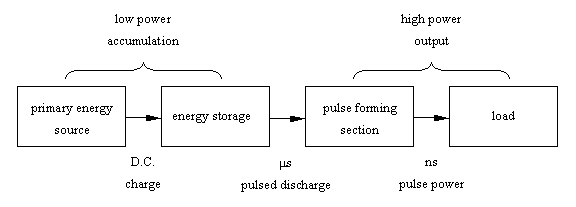
\includegraphics[height=4cm,width=8cm,keepaspectratio=true]{HPMsystem}
 \caption{Primjer ubacivanja slike}
 \label{fig:prva}
	\end{center}
\end{figure}

Znak \verb|~| iza rije�i Slici osigurava to�no jedan znak razmaka, �to poma�e ukoliko je rij�e Slika na kraju retka, da ne razdvoji rije� Slika i pripadaju�i broj slike.
Parametri slike \emph{width} i \emph{height} odre�uju maksimalne dopu�tene dimenzije pri �emu se primarno po�tuje manju navedenu dimenziju, a \emph{keepaspectratio} osigurava zadr�avanje odnosa dimenzija slike, odnosno sprje�ava deformaciju slike, nakon proizvoljno unesenih veli�ina.

Uo�i da sve oznake tj.\ \emph{labeli} ne smiju imati razmak u imenu. To vrijedi i op�enito, a ne samo za slike.

Tako�er, uo�i da nije potrebno pisati ekstenziju slike jer to je ure�eno u postavkama glavnoga dokumenta pa time �tedi trud. Ekstenzije koje se mo�e izostaviti su: \emph{jpg}, \emph{jpeg}, \emph{png} i \emph{pdf}.

Shema prikazana na Slici~\ref{fig:prva} �e biti kori�tena i za potrebe idu�ih primjera, a {\color{blue} u mapi na va�em disku ju obri�ite nakon �to po�nete pohranjivati vlastite slike vezane uz va� rad}.


\section{Ubacivanje podslika}
%
\begin{figure}[!htpb]
	  \begin{center}
	   \subfloat[kra�i opis podslike a]{\label{fig:HPM_a} 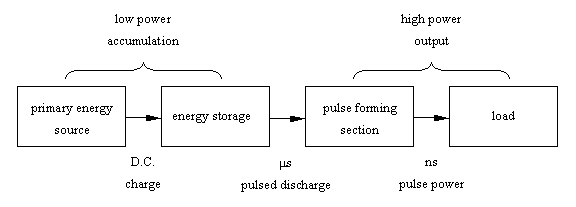
\includegraphics[height=5cm,width=8cm,keepaspectratio=true]{HPMsystem}} \\ %\hspace{10pt}
	   \subfloat[kra�i opis podslike b]{\label{fig:HPM_b} 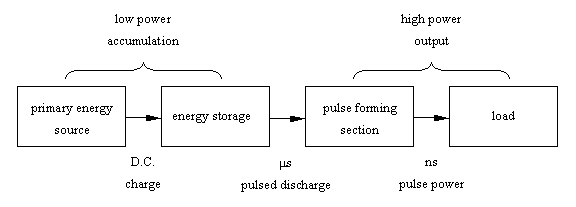
\includegraphics[height=5cm,width=8cm,keepaspectratio=true]{HPMsystem}}
\caption{Primjer ubacivanja vi�e podslika. Ovo je opis cijele slike.}
\label{fig:HPMsystem_2}
	  \end{center}
\end{figure}

Na Slici~\ref{fig:HPMsystem_2} su prikazane dvije podslike. 
Podslika~\ref{fig:HPM_a} pokazuje shemu HPM sustava, a podslika~\ref{fig:HPM_b} -- to isto.


\section{Ubacivanje tabele} \label{tabela}
Vi�e detalja o kreiranju tabela pro�itajte u literaturi, a sljede�i blok vam omogu�ava kreiranje jednostavne tabele, kao �to je prikazano u Tabeli~\ref{tab:prva}.
\begin{table}[!htbp]
\caption{Ovo je primjer izrade tabele}
\centering
\begin{tabular}{|c|c|c|}
\hline
variabla & vrijednost 1 & vrijednost 2  \\ [0.5ex]
\hline \hline  
A & 5 & 3 \\ [0.5ex]
B & 4 & 2 \\ [0.5ex]
\hline
\end{tabular}
\label{tab:prva}
\end{table}

Podaci koji su u stupcima se u tabeli razdvajaju znakom \&. Novi redak se na kraju aktualnoga retka formira znakom \verb|\\|. Broj stupaca se definira iza \emph{tabular} time �to se navedu slova koja ozna�avaju poravnavanje teksta u svakom stupcu, a broj slova zna�i broj stupaca koji �e biti kreiran u tabeli.


\section{Referenca na literaturu, sekciju, stranicu}
Na pojedinu se literaturu jednostavno uputi kori�tenjem naredbe \verb|\cite{bitex_key}| gdje je \emph{bibtex\_key} identifikator te bibliografske jedinice u bibtex datoteci. Npr.\ \verb|\cite{latex}| �e u tekstu pokazati broj te bibliografske jedinice u uglatoj zagradi \cite{latex}, te ju s istim brojem uvrsiti u popis literature (Bibliografiju) na kraju rada.

Ako se �elimo referirati na tekst u nekoj drugoj sekciji, kao npr. na dio gdje se opisuje kreiranje tabele, tada kraj te sekcije stavimo oznaku \verb|\label{ID}|, npr.\ \verb|\label{tabela}|, a na �eljenom mjestu u tekstu se na to referiramo pomo�u \verb|\ref{ID}|, npr.\ \verb|\ref{tabela}|. Tako mo�emo onda napisati da je kreiranje tabele opisano u Sekciji~\verb|~\ref{tabela}|, �to proizvede tekst koji glasi ``u Sekciji~\ref{tabela}''.

Ako �elimo navesti stranicu u na�em radu u kojoj se nalazi neki dio informacije o kojem govorimo, tada na isti na�in primijenimo \verb|\label{ID}| oznaku, a za referiranje na tu stranicu koristimo sintaksu \verb|\pageref{ID}|. 
Tako npr.\ mo�emo re�i da je primjer kreiranja tabele opisan na stranici~\verb|\pageref{tabela}|, �to �e za rezultat ima tekst u kojem pi�e da je primjer kreiranja tabele ``opisan na stranici~\pageref{tabela}''.

\section{Nagla�avanje teksta}
\subsection{Navodnici}
Za navodnike s lijeve strane fraze (otvaranje navodnika) koristi se 2x jednostruki navodnik koji se na tipkovnici nalazi lijevo od broja 1, a za navodnike s desne strane fraze (zatvaranja navodnika) se koristi 2x jednostruki navodnik koji se na tipkovnici nalazi na tipki \emph{�}, �to proizvede npr.\ ``abc''.

Alternativno, u ovom paketu je pripremljena i naredba \verb|\navod{abc}| gdje je \emph{abc} tekst koji se stavlja izme�u navodnika, tj.\ \navod{abc}.

\subsection{Kosa i podebljana slova}
Nagla�eni tekst (sli�no kosim slovima) mo�emo dobiti uporabom naredbe \verb|\emph{abc}| gdje je \emph{abc} neki tekst koji se �eli naglasiti.

Kosa slova (italic) mo�emo dobiti uporabom naredbe \verb|\textit{abc}| gdje je \textit{abc} neki tekst koji se �eli naglasiti.

Podebljana slova mo�emo posti�i uporabom naredbe \verb|\textbf{abc}| gdje je \textbf{abc} neki tekst koji �elimo podebljati.

\section{Verbatim okru�enje}
Verbatim okru�enje omogu�ava ispis teksta u izvornom obliku, bez da ga \LaTeX~ tuma�i po svojoj default sintaksi. To je pogodno kada se npr.\ na stranicu �eli kopirati dio programskoga koda iz nekog jezika i �elimo zadr�ati sve izvorne znakove, a ne da \LaTeX po�ne javljati pogre�ke kod kompajliranja jer �e ih bez toga interpretirati kao pogre�ke u sintaksi.

Postoji kra�i i du�i oblik verbatima. Kra�i slu�i za kra�u frazu od jedne ili par rije�i, a du�i za vi�e redaka.

Kra�i ima sintaksu: \verb+\verb|neka fraza|+

Du�i ima sintaksu:\\
\verb|\begin{verbatim}| \\
\verb|neki tekst| \\
\verb|\end{verbatim}| \\


\section{Kreiranje jedne jednad�be ili serije jednad�ba}

\subsection{Kreiranje jedne jednad�be}
Jednad�ba se napi�e u posebnom matemati�kom modu koji se kreira pomo�u bloka:
\begin{equation}
 A = B + C   \label{eq:prva}
\end{equation}

Jednad�ba~\eqref{eq:prva} je jedna jednostavna numerirana jednad�ba. Ako ju se ne �eli numerirati, onda se nakon rije�i \emph{begin} stavi zvjezdica, tj.\ \emph{begin\*}.

\subsection{Kreiranje vi�e jednad�ba}
Vi�e se jednad�ba kreira \emph{subequations} blokom:
\begin{subequations}
Dvije jednad�be mogu npr.\ glasiti:
\begin{align}
        A &= B + C  				\label{subeq:prva} \\
        D &= F + G				  \label{subeq:druga}
\end{align}
\label{subeq:obje}
\end{subequations}

U \eqref{subeq:prva} je prikazano dobivanje vrijednosti $A$, a u \eqref{subeq:druga} je prikazano dobivanje vrijednosti $D$. Jed.~\eqref{subeq:obje} je �uveni studentov zakon!

\section{Liste}
Liste su �este forme u tekstu kojima se na pregledni na�in nabrajaju neke stavke. Stavke obi�no navodimo s to�kama na po�etku, ili s brojevima ili sa slovima. U \LaTeX~u su upravo ta tri stila unaprijed definirana, a mogu�e su i slo�enije definicije stilova i kombinacije lista.

\subsection{Lista s to�kama}
Lista s to�kama se postigne blokom
\begin{verbatim}
\begin{itemize}
	\item prva stavka
	\item druga stavka
\end{itemize}
\end{verbatim}
�to na ekranu proizvede:
\begin{itemize}
	\item prva stavka
	\item druga stavka
\end{itemize}

\subsection{Numerirana lista s brojevima}
Numerirana lista s brojevima se postigne blokom
\begin{verbatim}
\begin{enumerate}
	\item prva stavka
	\item druga stavka
\end{enumerate}
\end{verbatim}
�to na ekranu proizvede:
\begin{enumerate}
	\item prva stavka
	\item druga stavka
\end{enumerate}


\subsection{Slov�ano numerirana lista}
Takva se lista mo�e posti�i u sklopu op�enitije forme koja omogu�uje proizvoljni opis ispred pojedine stavke, pomo�u sljede�ega bloka:
\begin{verbatim}
\begin{description}
	\item[a)] prva stavka
	\item[b)] druga stavka
\end{description}
\end{verbatim}
�to na ekranu proizvede:
\begin{description}
	\item[a)] prva stavka
	\item[b)] druga stavka
\end{description}



\section{Zavr�ne napomene}
Ovime zaklju�ujemo upute koje �e najve�em broju studenata biti dovoljne (ili barem dovoljna osnova) za uspje�no pisanje Zavr�noga odnosno Diplomskoga rada.

Prije nego prije�ete na kreiranje vlastitoga sadr�aja u�inite sljede�e:
\begin{enumerate}
	\item u mapi \href{run:slike}{{\color{blue}slike}}, obri�ite datoteku \verb|HPMsystem.png| jer je ona samo slu�ila za ilustracije u uputama
	%
	\item u glavnoj datoteci  \href{run:JMBAG\_Ime\_Prezime.tex}{{\color{blue}JMBAG\_Ime\_Prezime.tex}} stavite znak komentare ``\%'' ispred linije \verb|\include{Intro}| kojom se pozivaju ove upute, �ime to vi�e ne�e biti uklju�eno u tekst vlastitoga rada
	%
	\item otvorite datoteku \href{run:Poglavlje\_1.tex}{{\color{blue}Poglavlje\_1.tex}} i po�nite pisati svoj vlastiti tekst uz postavljanje naslova poglavlja i sekcija po vlastitom izboru, a na kraju promijenite ime te datoteke u ne�to �to odgovara sadr�aju va�ega poglavlja i to ime stavite u \verb|\include| naredbu umjesto inicijalnoga naziva \verb|Poglavlje_1|. Kona�no, da bi se tekst toga poglavlja kompajlirao u izlazni dokument, uklonite znak komentara ``\%'' ispred te \verb|\include| naredbe. Tako u�inite i za sva nova poglavlja koja �ete potom kreirati.
\end{enumerate}


Svoje dojmove o razumljivosti i prakti�nosti ovoga materijala mo�ete emailati klikom \href{mailto:mjoler@riteh.hr}{{\color{blue}ovdje}}.

Ugodan rad!


Miroslav Joler



%%%%%  POGLAVLJE ZAVRSENO  %%%%%| kojom se pozivaju ove upute, �ime to vi�e ne�e biti uklju�eno u tekst vlastitoga rada
	%
	\item otvorite datoteku \href{run:Poglavlje\_1.tex}{{\color{blue}Poglavlje\_1.tex}} i po�nite pisati svoj vlastiti tekst uz postavljanje naslova poglavlja i sekcija po vlastitom izboru, a na kraju promijenite ime te datoteke u ne�to �to odgovara sadr�aju va�ega poglavlja i to ime stavite u \verb|\include| naredbu umjesto inicijalnoga naziva \verb|Poglavlje_1|. Kona�no, da bi se tekst toga poglavlja kompajlirao u izlazni dokument, uklonite znak komentara ``\%'' ispred te \verb|\include| naredbe. Tako u�inite i za sva nova poglavlja koja �ete potom kreirati.
\end{enumerate}


Svoje dojmove o razumljivosti i prakti�nosti ovoga materijala mo�ete emailati klikom \href{mailto:mjoler@riteh.hr}{{\color{blue}ovdje}}.

Ugodan rad!


Miroslav Joler



%%%%%  POGLAVLJE ZAVRSENO  %%%%%| kojom se pozivaju ove upute, �ime to vi�e ne�e biti uklju�eno u tekst vlastitoga rada
	%
	\item otvorite datoteku \href{run:Poglavlje\_1.tex}{{\color{blue}Poglavlje\_1.tex}} i po�nite pisati svoj vlastiti tekst uz postavljanje naslova poglavlja i sekcija po vlastitom izboru, a na kraju promijenite ime te datoteke u ne�to �to odgovara sadr�aju va�ega poglavlja i to ime stavite u \verb|\include| naredbu umjesto inicijalnoga naziva \verb|Poglavlje_1|. Kona�no, da bi se tekst toga poglavlja kompajlirao u izlazni dokument, uklonite znak komentara ``\%'' ispred te \verb|\include| naredbe. Tako u�inite i za sva nova poglavlja koja �ete potom kreirati.
\end{enumerate}


Svoje dojmove o razumljivosti i prakti�nosti ovoga materijala mo�ete emailati klikom \href{mailto:mjoler@riteh.hr}{{\color{blue}ovdje}}.

Ugodan rad!


Miroslav Joler



%%%%%  POGLAVLJE ZAVRSENO  %%%%%   % ovo poslije staviti pod komentar kada se nau�i koristiti
%\chapter{Naslov poglavlja}

\section{Naslov sekcije}

\section{Naslov sekcije}

% itd.

%%%%  POGLAVLJE ZAVRSENO  %%%%%
  % dati neko logicno ime umjesto ``Poglavlje_1''
%\include{Poglavlje_2} 
%\include{Poglavlje_3} % itd.

% ispod \appendix zaglavlja pomocu \include dodati poglavlja s prilozima
\appendix
\chapter{Naslov priloga}

\section{Naslov sekcije}

\section{Naslov sekcije}

% itd.

%%%%  POGLAVLJE ZAVRSENO  %%%%%
  % dati neko suvislo ime umjesto ovoga
%\include{Prilog_2}  % itd.
%

%I) rucno upisati svaku referencu redoslijedom kojim se prvi puta pozivaju u tekstu
%\begin{thebibliography}{99}
%
%\bibitem{html} .....opis reference .........
%
%\bibitem{qwe} .......opis reference ........

%\bibitem{ajax}  .........opis reference..........
%
%\end{thebibliography}


%II) bolji nacin: pomocu programa JabRef opisati svoje reference i pohraniti u datoteku ``Literatura''. U tekstu samo pozivati zeljene reference, a lista se sama formira.
\bibliographystyle{tex_aux/IEEEtranHR}  % ``unsrt'', ``IEEEtran'', ``ieeetr''
% argument is your BibTeX string definitions and bibliography database(s)
\bibliography{Literatura}
  % ovo je ime Bibtex datoteke koju korisnik kreira


\end{document}
